\chapter{Discussion and Conclusion}
From the extensive study of energy resolution carried out in this project, we can make following conclusions from our observations for pions and electrons.

\begin{enumerate}
\item \textbf{Electrons:} EEMC shows excellent energy resolution behaviour since a crystal calorimeter is used. 
CEMC and FEMC also show better energy resolution than minimum expectations.
\item \textbf{Pions (Hadrons):} After handling mips, it is vivid that the energy resolution reaches the minimum expectations from the two calorimeter regions. In forward region, FEMC energies must be multiplied by a factor of 2 to obtain acceptable resolution behavior.

\end{enumerate}

\textbf{Future Scope of Work:}
\begin{enumerate}
    \item This study has been carried without digitization and noise in calorimeters. For future studies, it is advised to observe the changes in the calorimeter resolution upon introduction of noise.
    \item Another interesting study would be to study the tracking and calorimetry together to check the momentum along with energy response.
\end{enumerate}




















\begin{comment}

\begin{figure}[h!]
    \centering
    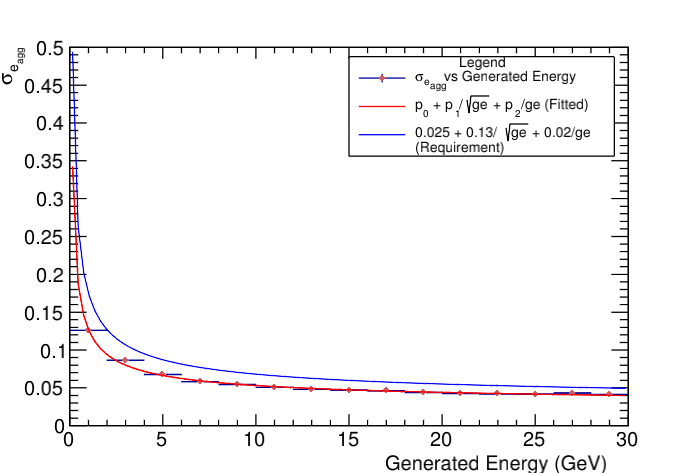
\includegraphics[width=\linewidth]{CEMC_sigmaE_ge_EtaCut_CircularCut.png}
    \caption{Energy Resolution of CEMC}
    \label{fig:CEMC}
\end{figure}

\begin{figure}[h!]
    \centering
    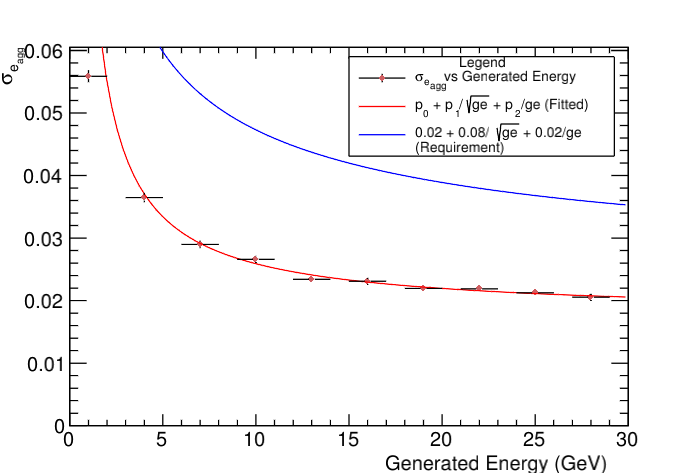
\includegraphics[width=\linewidth]{FEMC_Sigma.png}
    \caption{Energy Resolution of FEMC}
    \label{fig:FEMC}
\end{figure}

\begin{figure}[h!]
    \centering
    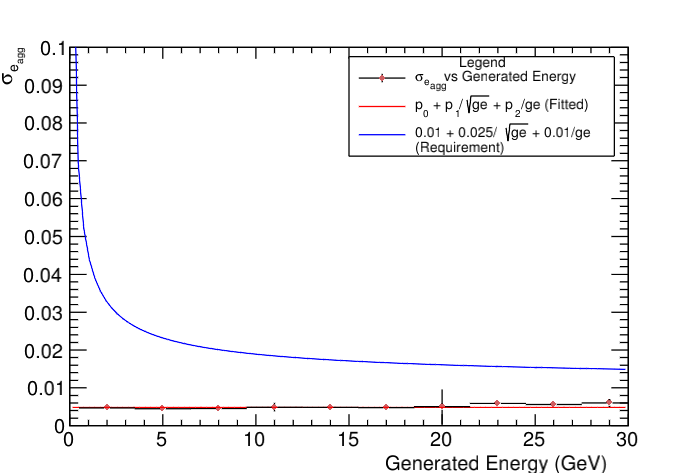
\includegraphics[width=\linewidth]{EEMC_Sigma.png}
    \caption{Energy Resolution of EEMC}
    \label{fig:EEMC}
\end{figure}
\end{comment}


\begin{comment}

\begin{figure}[h!]
    \centering
    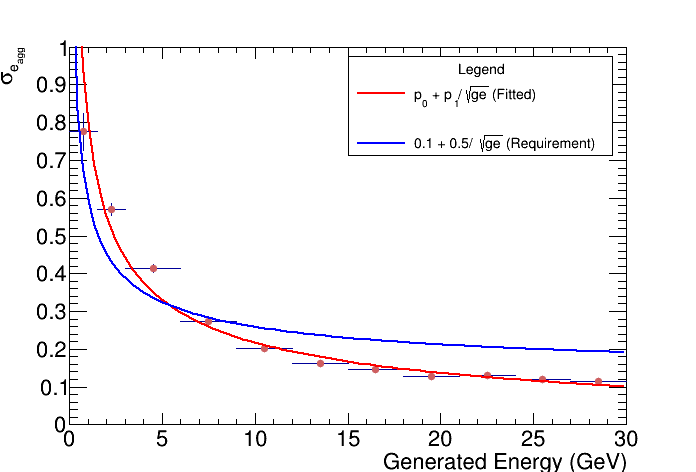
\includegraphics[width=\linewidth]{FHCAL_FEMC_sigmaE_ge_EtaCut_CircularCut.png}
    \caption{Energy Resolution of FEMC + FHCAL}
    \label{fig:Forward}
\end{figure}

\begin{figure}[h!]
    \centering
    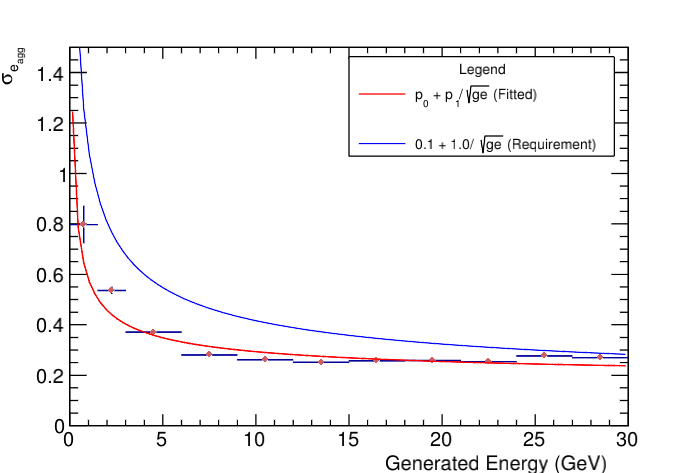
\includegraphics[width=\linewidth]{HCALIN_HCALOUT_CEMC_sigmaE_ge_EtaCut_CircularCut.png}
    \caption{Energy Resolution of CEMC + HCALIN + HCALOUT}
    \label{fig:Barrel}
\end{figure}
\end{comment}
